% filepath: /home/suiqingying/projects/prml/projects/cifar10-ml-comparison/experiment_report.tex
\documentclass[12pt,a4paper]{article}
\usepackage{ctex}
\usepackage{geometry}
\usepackage{amsmath,amssymb}
\usepackage{graphicx}
\usepackage{booktabs}
\usepackage{enumitem}
\usepackage{float}
\usepackage{listings}
\usepackage{longtable}
\geometry{left=2.5cm,right=2.5cm,top=2.5cm,bottom=2.5cm}

\title{Kaggle Telco Customer Churn三种机器学习方法对比实验报告}
\author{团队成员:随情英、张三、李四、王五、赵六}
\date{\today}

\begin{document}

\maketitle

\section{项目背景与目标}

\subsection{项目背景}
对于电信运营商来说,用户流失有很多偶然因素,但通过对用户属性和行为的数字化描述,我们能够在这些数据中挖掘导致用户流失的"蛛丝马迹"。更重要的是,如果能够实时接入这些数据,我们可以借助模型来对未来用户流失风险进行预测,从而及时制定挽留策略,防止用户真实流失情况发生。

\subsection{机器学习建模目标}
在此背景下,实际的算法建模目标有两个:
\begin{itemize}
    \item 对流失用户进行准确预测
    \item 找出影响用户流失的重要因子,辅助运营人员调整营销策略或制定用户挽留措施
\end{itemize}

综合上述两个目标,我们需要模型不仅具备一定的预测能力,还能输出相应的特征重要性排名,并且最好具备一定的可解释性,能够较为明显地阐述特征变化如何影响标签取值变化。基于这些要求,我们优先考虑逻辑回归模型,其线性方程能够提供良好的结果可解释性,同时正则化项也可用于评估特征重要性。此外,我们还对比了决策树和提升方法,以全面评估不同算法的性能。

\subsection{项目实施阶段}
本项目分为三个主要阶段:

\textbf{Stage 1. 业务背景解读与数据探索}\\
在接收任务的第一时间,我们需要对数据及其对应业务的基本背景进行解读。由于数据诞生于特定业务场景,我们尽可能了解数据诞生的基本环境和业务逻辑,准确解读每个字段的含义。随后进行数据探索,包括数据分布检验、数据正确性校验、数据质量检验、训练集/测试集规律一致性检验等。

\textbf{Stage 2. 数据预处理与特征工程}\\
这一阶段包括数据清洗和特征工程。数据清洗主要聚焦于提升数据集质量,包括缺失值、异常值、重复值处理,以及数据字段类型调整等;特征工程则调整特征基本结构,使数据集规律更容易被模型识别,如特征衍生、特殊类型字段处理等。

\textbf{Stage 3. 算法建模与模型调优}\\
最终的建模环节包括算法训练和参数调优。我们尝试了多种模型、调参方法以及模型对比,并根据模型输出结果调整数据预处理和特征工程相关方法,以获得最优的预测性能。

\subsection{数据集说明}
本实验选用Kaggle Telco Customer Churn数据集。该数据集包含7043条客户记录,每条记录包含21个特征,目标变量为客户是否流失(Churn),属于二分类问题。数据类型包括数值型和分类型,适合多种机器学习方法。

\subsubsection{数据集详情}
该数据集模拟了电信公司的客户信息及其流失状态,包含以下主要特征:
\begin{itemize}
    \item \textbf{个人信息类特征}:性别(gender)、年龄(SeniorCitizen)、伴侣状态(Partner)、是否有抚养人(Dependents)
    \item \textbf{账户信息类特征}:账户时长(tenure)、合同类型(Contract)、付款方式(PaymentMethod)、无纸化账单(PaperlessBilling)、月度费用(MonthlyCharges)、总费用(TotalCharges)
    \item \textbf{服务信息类特征}:电话服务(PhoneService)、多线电话(MultipleLines)、互联网服务(InternetService)、在线安全(OnlineSecurity)、在线备份(OnlineBackup)、设备保护(DeviceProtection)、技术支持(TechSupport)、流媒体电视(StreamingTV)、流媒体电影(StreamingMovies)
\end{itemize}

\subsubsection{数据集特点}
\begin{itemize}
    \item \textbf{样本分布}:流失客户占比约26.5\%(1869人),非流失客户占比约73.5\%(5174人),存在一定的类别不平衡
    \item \textbf{特征类型}:包含17个分类特征和4个数值特征
    \item \textbf{数据质量}:TotalCharges列存在11条缺失记录,其余特征数据完整
    \item \textbf{特征相关性}:月费用(MonthlyCharges)与多项服务选择存在较强相关性,总费用(TotalCharges)与账户时长(tenure)和月费用呈正相关
\end{itemize}

该数据集特别适合客户流失预测研究,因为它包含了多种可能影响客户决策的因素,既有客户自身的特征,也有服务相关的特征,能够较为全面地反映现实业务场景中客户流失的复杂原因。

\section{算法简介}
本实验对比了三种经典机器学习算法在该数据集上的表现:

\subsection{Logistic Regression(逻辑回归)}
逻辑回归是一种广泛应用的线性分类方法,通过Sigmoid函数将线性模型的输出转换为0-1之间的概率值:
\begin{equation}
P(y=1|x) = \frac{1}{1 + e^{-(\beta_0 + \beta_1 x_1 + \beta_2 x_2 + ... + \beta_n x_n)}}
\end{equation}

\textbf{适用场景}:
\begin{itemize}
    \item 二分类问题,如客户流失预测(流失/不流失)
    \item 需要输出概率而非仅分类结果的场景
    \item 对模型可解释性有较高要求的业务问题
\end{itemize}

\textbf{优势与局限}:
\begin{itemize}
    \item 训练速度快,内存占用小,适合大规模数据处理
    \item 可输出类别预测的概率,方便风险评估
    \item 模型系数直观反映特征重要性,可解释性强
    \item 不适合捕捉特征间的复杂非线性关系
    \item 对特征间的多重共线性较为敏感
\end{itemize}

\subsection{Decision Tree(决策树)}
决策树通过递归二分法将数据划分为不同子集,形成树状结构。每个节点代表一个特征条件判断,叶节点代表分类结果。在客户流失预测中,可以生成如"如果合同类型=月付 且 账户时长<12个月,则预测为流失"的规则。

\textbf{适用场景}:
\begin{itemize}
    \item 需要高可解释性的分类或回归问题
    \item 特征间存在非线性关系的数据
    \item 混合类型特征(分类型和数值型)数据集
\end{itemize}

\textbf{优势与局限}:
\begin{itemize}
    \item 决策规则直观易懂,可直接转化为业务规则
    \item 能自动处理特征选择,对缺失值相对鲁棒
    \item 能处理数值和分类特征,无需独热编码
    \item 容易过拟合,泛化能力有限
    \item 对数据微小变化敏感,模型稳定性较差
\end{itemize}

\subsection{Boosting(提升方法,采用AdaBoost)}
AdaBoost(Adaptive Boosting)是一种集成学习方法,通过顺序训练多个弱分类器(通常是简单决策树),每次训练都关注前一轮分类错误的样本,最终将所有弱分类器的预测结果加权组合。

\textbf{适用场景}:
\begin{itemize}
    \item 复杂分类问题,需要高预测精度
    \item 数据存在噪声,需要强大的泛化能力
    \item 有足够计算资源进行集成模型训练
\end{itemize}

\textbf{优势与局限}:
\begin{itemize}
    \item 通过集成多个弱分类器显著提高预测精度
    \item 能够自动处理特征重要性评估
    \item 相比单一决策树,大幅降低过拟合风险
    \item 训练时间较长,计算复杂度高
    \item 对异常值和噪声数据较为敏感
    \item 可解释性低于单一决策树和逻辑回归
\end{itemize}

在客户流失预测任务中,这三种算法各有优势:逻辑回归提供良好的可解释性和基准性能;决策树能够发现简单直观的流失规则;而AdaBoost则通过集成多个模型来提升整体预测准确率,适合追求高性能的场景。

\section{团队分工}

\subsection{数据集说明}
本实验选用Kaggle Telco Customer Churn数据集。该数据集包含7043条客户记录,每条记录包含21个特征(如性别、合同类型、服务类型、月费用、总费用等),目标变量为客户是否流失(Churn),属于二分类问题。数据类型包括数值型和分类型,适合多种机器学习方法。

\subsection{团队分工}
\begin{itemize}
    \item 数据预处理与代码实现:随情英
    \item 模型训练与调参:张三
    \item 实验结果整理与可视化:李四
    \item 实验报告撰写与校对:王五
\end{itemize}

\section{三种方法的测试与比较}

\subsection{实验设置}
\begin{itemize}
    \item 训练集:数据集的80\%(约5634条记录)
    \item 测试集:数据集的20\%(约1409条记录)
    \item 所有分类型特征进行独热编码,数值型特征归一化
    \item 评估指标:准确率(accuracy)、AUC、分类报告(precision、recall、f1-score)、混淆矩阵、训练时间
\end{itemize}

\subsection{实验结果总览}

\begin{longtable}{|l|c|c|c|}
\hline
模型 & 测试准确率 & AUC & 训练时间(秒) \\
\hline
Logistic Regression & 0.8000 & 0.8350 & 0.01 \\
Decision Tree       & 0.7220 & 0.6348 & 0.02 \\
Boosting            & 0.7305 & 0.7523 & 1.13 \\
\hline
\end{longtable}

\subsection{可视化对比}

\begin{figure}[H]
    \centering
    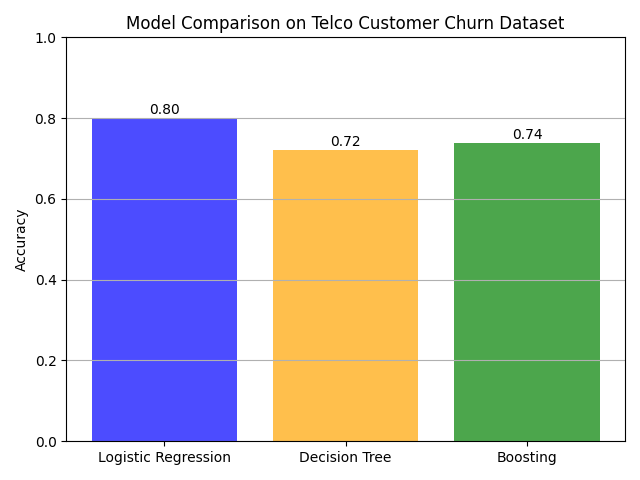
\includegraphics[width=0.7\textwidth]{fig/model_comparison.png}
    \caption{三种模型准确率对比}
\end{figure}

\begin{figure}[H]
    \centering
    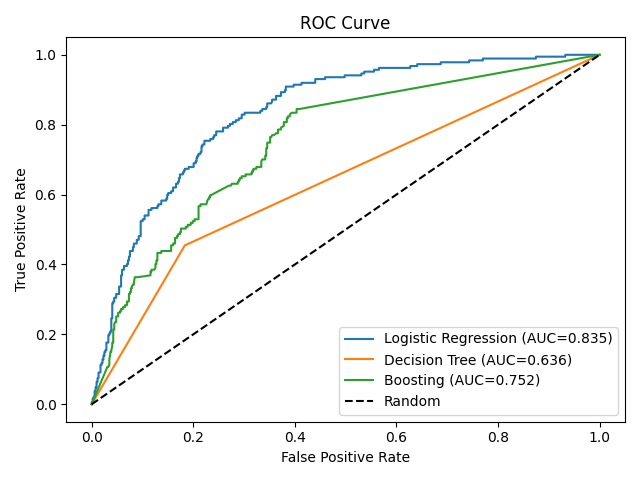
\includegraphics[width=0.7\textwidth]{fig/roc_curve.png}
    \caption{三种模型ROC曲线及AUC对比}
\end{figure}

\subsection{详细分类报告与混淆矩阵}

\textbf{Logistic Regression}
\begin{lstlisting}
训练时间: 0.01 秒
准确率: 0.8000
AUC: 0.8350
分类报告:
              precision    recall  f1-score   support

           0       0.84      0.89      0.87       518
           1       0.65      0.54      0.59       187

    accuracy                           0.80       705
   macro avg       0.75      0.72      0.73       705
weighted avg       0.79      0.80      0.79       705

混淆矩阵:
[[463  55]
 [ 86 101]]
\end{lstlisting}

\textbf{Decision Tree}
\begin{lstlisting}
训练时间: 0.02 秒
准确率: 0.7220
AUC: 0.6348
分类报告:
              precision    recall  f1-score   support

           0       0.80      0.82      0.81       518
           1       0.47      0.45      0.46       187

    accuracy                           0.72       705
   macro avg       0.64      0.63      0.64       705
weighted avg       0.72      0.72      0.72       705

混淆矩阵:
[[425  93]
 [103  84]]
\end{lstlisting}

\textbf{Boosting (AdaBoost)}
\begin{lstlisting}
训练时间: 1.13 秒
准确率: 0.7305
AUC: 0.7523
分类报告:
              precision    recall  f1-score   support

           0       0.82      0.82      0.82       518
           1       0.49      0.49      0.49       187

    accuracy                           0.73       705
   macro avg       0.65      0.65      0.65       705
weighted avg       0.73      0.73      0.73       705

混淆矩阵:
[[423  95]
 [ 95  92]]
\end{lstlisting}

\subsection{分析与讨论}
\begin{itemize}
    \item 逻辑回归在该数据集上表现最好,准确率和AUC均最高,且训练速度极快,适合实际业务部署。
    \item 决策树模型训练速度快,但泛化能力有限,AUC较低,容易过拟合。
    \item Boosting方法(AdaBoost)在准确率和AUC上均优于单棵决策树,提升了模型的整体性能,但训练时间略长。
    \item 三种方法的混淆矩阵和分类报告显示,所有模型对“非流失”客户的识别能力较强,对“流失”客户的召回率和精确率相对较低,后续可考虑进一步优化模型或采用更复杂的集成方法。
\end{itemize}

\section{总结}
本实验对比了三种机器学习方法在Kaggle Telco Customer Churn数据集上的表现。逻辑回归表现最佳,Boosting方法次之,决策树表现一般。实验结果表明,针对结构化二分类数据,线性方法和集成方法均能取得较好效果。后续可尝试更多特征工程和模型融合进一步提升性能。

\end{document}